\documentclass[11pt,a4wide]{article}
\usepackage[dvips]{graphicx}
\usepackage{mathrsfs}
\usepackage{amsfonts}
\usepackage{lscape}

\usepackage{epic,eepic}
\usepackage{amsmath}
\usepackage{amssymb}
\usepackage[dvips]{epsfig}
\usepackage[T1]{fontenc}
\usepackage{hyperref}
\usepackage{bezier}
\usepackage{pstricks}
\usepackage{dcolumn}% Align table columns on decimal point
\usepackage{bm}% bold math
%\usepackage{braket}
\usepackage[dvips]{graphicx}
\usepackage{pst-plot}
\usepackage{colortbl}
%\usepackage[english]{babel}
\usepackage{listings}
\usepackage{shadow}
\lstset{language=c++}
\lstset{basicstyle=\small}
%\lstset{backgroundcolor=\color{white}}
%\lstset{frame=single}
\lstset{stringstyle=\ttfamily}
%\lstset{keywordstyle=\color{red}\bfseries}
%\lstset{commentstyle=\itshape\color{blue}}
\lstset{showspaces=false}
\lstset{showstringspaces=false}
\lstset{showtabs=false}
\lstset{breaklines}

\newcommand{\One}{\hat{\mathbf{1}}}
\newcommand{\eff}{\text{eff}}
\newcommand{\Heff}{\hat{H}_\text{eff}}
\newcommand{\Veff}{\hat{V}_\text{eff}}
\newcommand{\braket}[1]{\langle#1\rangle}
\newcommand{\Span}{\operatorname{sp}}
\newcommand{\tr}{\operatorname{trace}}
\newcommand{\diag}{\operatorname{diag}}
\newcommand{\bra}[1]{\left\langle #1 \right|}
\newcommand{\ket}[1]{\left| #1 \right\rangle}
\newcommand{\element}[3]
    {\bra{#1}#2\ket{#3}}

\newcommand{\normord}[1]{
    \left\{#1\right\}
}


\usepackage{amsmath}





\begin{document}

\title{Project 1,  PHY981 Spring 2016}
%\author{}
\maketitle
\section*{Project 1, Deadline March 4}


We are going to study a schematic model (the Lipkin model, Nucl.
Phys. {\bf 62} (1965) 188) for the interaction among $4$ fermions that
can occupy two different energy levels.  Although the model is simple,
it contains several ingredients relevant for nuclear structure, from
the handling of angular momenta using lowering and raising operators,
to a typical diagonalization problem with close similarities with
shell-model calculations. The project ends also with a Hartree-Fock
calculation which can be done analytically.  I would claim that if you understand the basic workings
of this model, irrespective of its simplicity, you should be able to
gain some of the underlying philosophy of how we interpret shell-model
data.  You can hand in your answer electronically (pdf, ps, ipython notebook, scanned
notes or your prefered document format) or just your handwritten notes.

The first part of the project involves a (slightly tedious) rewrite of various operators in terms of angular momentum 
operators. Here you need to play with various anti-commutation relations. The remaining part involves diagonalization of a $5\times 5$ Hamiltonian matrix, Hartree-Fock theory and discussion and analysis of your results.
There is also an optional part that gives you an additional score of 30\%. There the aim is to write a Hartree-Fock program which can be benchmarked against the closed form answers in exercise e). 
You are obviously free to collaborate with fellow students (I actually encourage that).  You can then hand in a common report. Groups of 2-3 students are often the optimal size. Good luck to you all! 

We have four fermions and 
each level has degeneration $d=4$. The two levels have quantum numbers $\sigma=\pm 1$,
with the upper level having  $\sigma=+1$ and energy
$\varepsilon_{1}=
\varepsilon/2$. The lower level  has $\sigma=-1$ and energy
$\varepsilon_{2}=-\varepsilon/2$. 
In addition, the substates  of each level are characterized  
by the quantum numbers $p=1,2,3,4$.  

We define the single-particle states
\[
\ket{u_{\sigma =-1,p}}=a_{-p}^{\dagger}\ket{0}
\hspace{1cm}
\ket{u_{\sigma =1,p}}=a_{+p}^{\dagger}\ket{0}.
\]
The single-particle states span an orthonormal basis.
The Hamiltonian of the system is given by
\[
\begin{array}{ll}
H=&H_{0}+H_{1}+H_{2}\\
&\\
H_{0}=&\frac{1}{2}\varepsilon\sum_{\sigma ,p}\sigma
a_{\sigma,p}^{\dagger}a_{\sigma ,p}\\
&\\
H_{1}=&\frac{1}{2}V\sum_{\sigma ,p,p'}
a_{\sigma,p}^{\dagger}a_{\sigma ,p'}^{\dagger}
a_{-\sigma ,p'}a_{-\sigma ,p}\\
&\\
H_{2}=&\frac{1}{2}W\sum_{\sigma ,p,p'}
a_{\sigma,p}^{\dagger}a_{-\sigma ,p'}^{\dagger}
a_{\sigma ,p'}a_{-\sigma ,p}\\
&\\
\end{array}
\]
where $V$ and $W$ are constants. The operator 
$H_{1}$ can move pairs of fermions as shown in Fig.~(a)
while $H_{2}$ is a spin-exchange term.
As shown in Fig.~(b),
$H_{2}$ moves a pair of fermions from a state $(p\sigma ,p' -\sigma)$ to a state
$(p-\sigma ,p'\sigma)$.
\begin{figure}[hbtp]
\includegraphics[width=1.0\textwidth]{fig1.ps}
\end{figure}\newline
\begin{enumerate}
\item[a)] Introduce the quasispin operators
\[
\begin{array}{ll}
J_{+}=&\sum_{p}
a_{p+}^{\dagger}a_{p-}\\
&\\
J_{-}=&\sum_{p}
a_{p-}^{\dagger}a_{p+}\\
&\\
J_{z}=&\frac{1}{2}\sum_{p\sigma}\sigma
a_{p\sigma}^{\dagger}a_{p\sigma}\\
&\\
J^{2}=&J_{+}J_{-}+J_{z}^{2}+2\imath J_{z}\\
&\\
\end{array}
\]
Show that these operators obey the commutation relations for angular momentum (you need to look up a textbook in quantum mechanics here or chapter 1 of Suhonen).\newline
\item[b)] Express $H$ in terms of the above quasispin operators and the number operator
\[
N=\sum_{p\sigma}
a_{p\sigma}^{\dagger}a_{p\sigma}.
\]
\item[c)] Show that $H$ commutes with $J^{2}$, viz., $J$ is a good quantum number.\newline
\item[d)] Consider thereafter a state with all four fermions in the lowest level (see the above figure).
We can write this state as
\[
\ket{\Phi_{J_z=-2}} =a_{1-}^{\dagger}a_{2-}^{\dagger}
a_{3-}^{\dagger}a_{4-}^{\dagger}\ket{0}.
\]
This state has $J_{z}=-2$ and belongs to the set of possible projections of 
$J=2$. We introduce the shorthand notation
$\ket{J,J_z}$ for states with different values of
spin $J$ and its projection $J_z$.

The other possible values are  $J_{z}=-1$, $J_{z}=0$, $J_{z}=1$
and $J_{z}=2$. 
Use the ladder operators
$J_{+}$ and $J_{-}$  to set up the states 
with spin $J_{z}=-1$ $J_{z}=0$, $J_{z}=1$
and $J_{z}=2$.  
The action of these operators on a state with given spin 
$J$ and $J_z$ is  (with $\hbar = 1$) 
\[
J_+\ket{J,J_z}=\sqrt{J(J+1)-J_z(J_z+1)}\ket{J,J_z+1}
\] 
and
\[
J_-\ket{J,J_z}=\sqrt{J(J+1)-J_z(J_z-1)}\ket{J,J_z-1},
\] respectively.
\newline
\item[e)] Use thereafter the quasispin operators to construct the Hamiltonian matrix 
$H$ for this five-dimensional space.  Find the eigenvalues
(numerically using for example python, matlab or mathematica. If you need an eigenvalue solver for C++ or Fortran, let me know.)  for the following parameter sets:
\[
\begin{array}{cccc}
(1)&\varepsilon=2,&V=-1/3,&W=-1/4\\
(2)&\varepsilon=2,&V=-4/3,&W=-1
\end{array}
\]
Which state is the ground state? Comment and discuss your results.\newline
\item[f)]
The single-particle states for the 
 Lipkin model
\[
\ket{u_{\sigma =-1,p}}=a_{-p}^{\dagger}\ket{0}
\hspace{1cm}
\ket{u_{\sigma =1,p}}=a_{+p}^{\dagger}\ket{0}
\]
can now be used as basis for a new single-particle state
$\ket{\phi_{\alpha ,p}}$  via a unitary  transformation
\[
\ket{\phi_{\alpha ,p}}=
\sum_{\sigma =\pm1}C_{\alpha\sigma}\ket{u_{\sigma ,p}}
\]
with $\alpha=\pm 1$ og $p=1,2,3,4$. Why is $p$ the same in 
$\ket{\phi}$
as in $\ket{u}$?  Show that the new basis is orthonormal.
The approximation here mimicks the procedure for a Hartree-Fock calculation. 
\newline
\item[g)] With the new basis we can construct a new Slater determinant given by
$\ket{\Psi}$
\[
\ket{\Psi}=\prod_{p=1}^{4}b_{\alpha ,p}^{\dagger}\ket{0}
\]
with $b_{\alpha ,p}^{\dagger}\ket{0}=\ket{\phi_{\alpha ,p}}$. Use this Slater determinant to calculate
\[
E=\bra{\Psi}H\ket{\Psi},
\]
as a function of the coefficients $C_{\sigma\alpha}$. We assume that the coefficients are real.\newline
\item[h)] Show that
\[
  \frac{\epsilon}{3} > V+W,
\]
has to be fulfilled in order to find a minimum in the energy.
Hint: calculate the functional derivative  of the energy with respect to the coefficients $C_{\sigma\alpha}$. In this case you can find an analytical result for the variational minimum. We will call this for our Hartree-Fock results.

Discuss your results and give an interpretation of the Hartree-Fock results with respect to those obtained
by the exact diagonalization above. How would you interpret the Hartree-Fock results?


\end{enumerate}
\end{document}



